\section{Examples}\label{sec:examples}



\subsection{Concurrent Spanning Tree}\label{subsec:CST-example}
Programs manipulating arbitrary graphs present the following significant
challenge for compositional verification: because of deep sharing
between different components of a graph, changes to one subgraph may
affect other subgraphs which may point into it. This makes it hard to
reason about updates to each subgraph in isolation. In a concurrent
setting, this difficulty compounds with the fact that threads working
on different parts of the graph may affect each other in ways that are
difficult to reason about locally to each subgraph. Central to those
issues is the fact that different subgraphs present \emph{unspecified
  sharing} and may overlap in arbitrary ways. We now demonstrate on a
concurrent spanning tree example that \colosl may be just the tool needed in this case, as it naturally deals with arbitrary overlapping
views of the shared state, and allows one to tailor interferences to a
given subjective view.

Our example, presented in \fig\ref{fig:conSpanningTree}, operates on a
\emph{directed binary graph} (henceforth simply \emph{graph}),
i.e.\ a directed graph where each node has at most two
successors, called its left and right children. The program concurrently computes an
in-place spanning tree of the graph (i.e.\ a tree that covers
all nodes of the graphs from a given root), as follows:
each time a new node is encountered, two new threads are created that
each prune the edges of the left and right children recursively. A
mark bit is associated with each node to keep track of which ones have
already been visited. Each thread returns whether the root
of the subgraph it was operating on had already been visited; if so,
the parent thread removes the link from its root node to the
corresponding child. Intuitively, it is allowed to do so as the child has to be
already reachable via some other path in the graph since it was marked by another thread.

%% marking the vertices to keep track of those already visited; the
%% return value b records the outcome of marking with \li{b}$=1$ when the
%% top node $x$ is unmarked (not visited yet) and \li{b}$=0$
%% otherwise. Assuming that the root vertex $x$ is unmarked initially,
%% the algorithm continues by first marking $x$ and subsequently spanning
%% the left and right subgraphs concurrently. When the top node of the
%% left subgraph is already marked (\li{!b1}), the edge from $x$ into it
%% is replaced by a null pointer. This corresponds to the case where the
%% node has already been visited by another thread and is thus reachable
%% from the root; \emph{mutatis mutandis} for the right subgraph.

We will prove that, given a shared graph as input, the program always
returns a tree, i.e.\ all sharing and cycles have been
appropriately removed. Pleasingly, the \colosl specification achieves
maximal locality and allows us to reason only on the current subgraph
manipulated by a thread, instead of the whole graph. Because of
arbitrary sharing between the two, a global specification would be
unpleasant indeed. 
%However, we do not establish that the final tree
%indeed spans the original graph. The reason it does is subtle indeed,
%as are the invariants required, but in ways unrelated to our main
%issue, which is to provide tight specifications for each thread.

To reason about this program, following~\cite{ramification} we use two representations of graphs. The
first is a mathematical representation $\gamma = (V, E)$ where $V$ is
a finite set of vertices and $E: V \rightarrow (V \uplus
\{\li{null}\}) \times (V \uplus \{\li{null}\})$ is a function
associating each vertex with at most two successors, where \li{null}
denotes the absence of a child.  We write $n \in \gamma$
for $n \in V$, $\gamma(n)$ for $E(n)$ and $|\gamma|$ for $|V|$.

Mathematical graphs are connected to their in-memory representations
by an inductive predicate $\graph{x}{\gamma}$, denoting a spatial
(in-heap) graph rooted at address $x$ corresponding to the
mathematical graph $\gamma$. The predicate defined in
\fig~\ref{fig:globalCST} uses the overlapping conjunction to account
for the sharing between the left and right children and for potential
cycles in the graph.  The basic
action we allow on spatial graphs is to \emph{mark} a node, changing
its mark field from $0$ to $1$ and claiming ownership of its left and
right pointers in the process. Such an action is allowed by a
\emph{marking} capability of the form $\markT{n}{e}$ where $n$ denotes
the vertex (address) and $e$ the edge via which vertex $n$ is visited.
Thus owning an unmarked vertex grants the right to visit and mark its
unmarked children, and the capabilities owned on a same node by
multiple threads do not clash because they would have gotten to that
node via different paths which yield different capabilities. For
instance, the capabilities associated with marking of vertex $z$ in
\fig\ref{fig:graphAndTree} are $\markT{z}{y.r}$ and
$\markT{z}{w.l}$. Note that the parameterisation of our actions are
merely a notational convenience and can be substituted for their full
definitions. In order to account for the ability to mark the root
vertex $x$ of a graph, we introduce a logical (virtual) root edge
$\rootEdge$ into $x$ as depicted in \fig\ref{fig:graphAndTree}
together with its associated marking capability
$\markT{x}{\rootEdge}$. The shared state contains node $x$ which can
be either unmarked ($\unmarked{x}{l}{r}$) or marked ($\marked{x}$); as
well as the left and right subgraphs represented recursively by
$\G{l}{\gamma}$ and $\G{r}{\gamma}$.
%% Note that the two subgraphs and vertex $x$ are combined by
%% the overlapping conjunction $\sepish$ since the graph can be cyclic
%% and each node may be reachable via more than one path.
%
%\begin{wrapfigure}[8]{r}{0.25\textwidth}
%	\centering
%	\begin{tabular}{|c |}
%		\hline
%			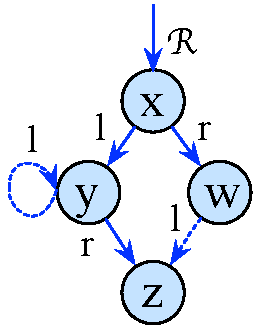
\includegraphics[scale=0.27]{Sections/Examples/Images/graph.pdf} \\
%		\hline
%	\end{tabular}
%\caption{A graph.}
%\label{fig:graphAndTree}
%\end{wrapfigure}
%%%
Each vertex is represented as three consecutive cells in the heap
tracking the mark bit and the addresses of the left ($l$) and right
($r$) subgraphs. We write $\cell{x}{m, l, r}$ for
$\cell{x}{m} * \cell{x+1}{l} * \cell{x+2}{r}$, and $x.m$, $x.l$, and
$x.r$ for $x$, $x+1$, and $x+2$, respectively. When vertex $x$ is in
the unmarked state, the whole cell $\cell{x}{0,l,r}$ and the
capabilities to mark the children reside in the shared state. In the
marked state, the shared state only contains $\cell{x.m}{1}$: the left
and right subgraphs (pointers and capabilities) have been claimed by
the thread who marked the node, while other threads need not access
the children of $x$ once they see that $x$ is already marked. The
atomic \li{CAS} (compare-and-swap) instruction prevents several threads to concurrently
mark the same node and claim ownership of the same resource.

The interference associated with the graph is described as the union
of interferences pertaining to the vertices of the graph ($n \in
\gamma$). For each vertex $n \in \gamma$, the only permitted action is
that of marking $n$ which can be carried out by any of the marking
capabilities associated with node $n$ ($\markT{n}{-}$). Note that the
anonymous quantification $-$ is yet another notational shorthand and
can be substituted for the following more verbose definition.\vspace*{-7pt}
%
\[
I(n) \eqdef
\{ \markT{n}{e} : \exsts{l, r} \unmarked{n}{l}{r} \swap \marked{n}
\mid e \in \{p.l,
  p.r, \rootEdge\} /| p \in \gamma\}
\]

\begin{figure}
 %\centering
%  \hspace*{0.2cm}
  \begin{minipage}{0.98\linewidth}
    \begin{tabular}{| c | l |}
    \hline	
    %\hspace*{-0.4cm}
    \begin{subfigure}[b]{0.14\textwidth}			
      \centering	
      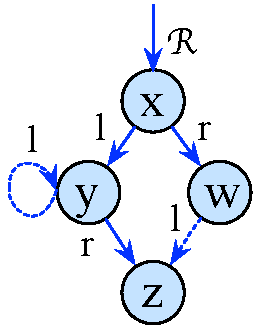
\includegraphics[scale=0.35]{Sections/Examples/Images/graph.pdf}\vspace*{5pt}\\
    \caption{}
    \label{fig:graphAndTree}
    \end{subfigure}
    &
    \begin{subfigure}[b]{0.86\textwidth}	\vspace{5pt}		
    $\begin{array}{@{\hspace{10pt}} r @{\hspace*{2pt}} l}
			\graph{x}{\gamma} \eqdef & \left[\markT{x}{\rootEdge}\right] * \shared{\G{x}{\gamma}}{I_\gamma} \hspace*{0.5cm} I_\gamma \eqdef \bigcup\limits_{n \in \gamma}I(n)\\
%	
			\G{x}{\gamma} \eqdef & (x = \li{null} \land \emp) \lor x \in \gamma \land \exsts{l, r} \gamma(x) = (l, r) \\
			& \land \left( \unmarked{x}{l}{r} \lor \marked{x}\right) \sepish \G{l}{\gamma} \sepish \G{r}{\gamma}\\
%
			\unmarked{x}{l}{r} \eqdef & \cell{x}{0, l, r} * \left[\markT{l}{x.l}\right] * \left[\markT{r}{x.r} \right]
			\qquad
			\marked{x} \eqdef  \cell{x}{1}\\
%
			I(n) \eqdef & \left\{ \markT{n}{-}: \exsts{l, r} \unmarked{n}{l}{r} \swap \marked{n}\right\}
		\end{array}
		$
		 \caption{}
    \label{fig:globalCST}
    \end{subfigure}\\
    \hline
    \end{tabular}
    %\caption{Abstract (de)allocation in SSL}
    \label{fig:graph-and-globalCST}	
  \end{minipage}
\caption{A binary graph (left); global specification of the graph predicate (right).}
\end{figure}

\begin{figure}
\hrule
\[
\begin{array}{r @{\hspace*{2pt}} l}
	\g{x}{\gamma} \eqdef & (x = \li{null} \land \emp) \lor x \in \gamma \land \exsts{l, r} \gamma(x) = (l, r) \land\\
	& \shared{\unmarked{x}{l}{r} \lor \marked{x}}{I(x)} * \g{l}{\gamma} * \g{r}{\gamma}\\
	
	\tr{x}{\gamma} \eqdef & (x = \li{null} \land \emp) \lor (x \in \gamma \land \exsts{l, r} \gamma(x) = (l, r) \land \exsts{l' \in \{l, \li{null}\}} \exsts{r' \in \{r, \li{null}\}}\\
	& \shared{\marked{x}}{I(x)} *
	\left[\markT{l}{x.l}\right] * \cell{x.l}{l'} * \tr{l'}{\gamma} * 
	\left[\markT{r}{x.r}\right] * \cell{x.r}{r'} * \tr{r'}{\gamma})
\end{array}
\]
\hrule
\caption{Local specification of the graph predicate.}
\label{fig:localCST}
\end{figure}

The $\graph{x}{\gamma}$ predicate defined in \fig\ref{fig:globalCST}
is a \emph{global} account of the graph in that it captures all
vertices and the interference associated with them. However, our
spanning tree algorithm operates \emph{locally} as it is called upon
recursively for each node. That is, for each \li{span(n)} call (where
$\cell{\li{n}}{n}$ and $n \in \gamma$), the footprint of the call is
limited to the subgraph rooted at $n$. Moreover, in order to reason about the concurrent recursive calls $\li{span(x.l)} || \li{span(x.r)}$, we need to \emph{split} the state into two $*$-composed states prior to the calls, pass each constituent state onto the relevant thread and combine the resulting states by $*$ composition through an application of the \parRule\ rule. We thus provide a \emph{local} specification of the graph, $\g{x}{\gamma}$ as defined in \fig\ref{fig:localCST} such that for all $n, p \in \gamma$ and $e \in \{p.l, p.r, \rootEdge \}$.\vspace{-7pt}
%
\[
\begin{array}{@{} c @{} }
	\color{blue}{
	\Big\{
		\cell{\li{n}}{n} * \cell{\li{b}}{-} * 
		\left[\markT{n}{e}\right] * 
		\g{n}{\gamma}
	\Big\} 
	} \\
%	
	\command{b:= span(n)} \\ 
%
	\color{blue}{
	\Big\{
		\cell{\li{n}}{n} *  
		\left[\markT{n}{e}\right] * 
		\left(
%		\begin{array}{@{} l @{}}
			\cell{\li{b}}{1} * \tr{n}{\gamma} \lor
			\cell{\li{b}}{0} *  \tr{\li{null}}{\gamma}
%		\end{array}
		\right)
	\Big\}
	}
\end{array}\vspace*{-7pt}
\]
%
The definition of the $\g{x}{\gamma}$ predicate is similar to that of
$\shared{\G{x}{\gamma}}{I_{\gamma}}$ except that the global view
$\shared{\G{x}{\gamma}}{I_{\gamma}}$ that describes the resources
associated with all $|\gamma|$ vertices has been broken down into more
local views, each attached to a vertex $n \in \gamma$. Moreover, the interference of each local view concerning a vertex $n \in \gamma$ has been shifted from $I_{\gamma}$ to $I(n)$ as to reflect only those actions that affect $n$.  

Similarly, the $\tr{x}{\gamma}$ predicate represents a \emph{tree}
rooted at $x$, as is standard in separation logic~\cite{rey02}, and
consists (once fully unfolded) of $|\gamma|$ subjective views one for each vertex in
$\gamma$. The assertion of each subjective view reflects that the
corresponding vertex ($x$) has been marked
$\shared{\marked{x}}{I(x)}$. The resources associated with each node
$x$, namely the left and right pointers and the corresponding marking
capabilities, have been claimed by the marking thread and moved into
its local state. The vertex addressed by the left pointer of $x$
(i.e.\ $l'$) corresponds to either the initial value prior to
marking ($l$ where $\gamma(x) = (l, r)$) or \li{null}\ when $l$ has
more than one predecessors and has been marked by another thread,
making the whole predicate stable against actions of the program and
the environment.

We now demonstrate how to obtain the local specification $\g{x}{\gamma}$ from the global specification of \fig\ref{fig:globalCST}. 
When expanding the definition of $\G{x}{\gamma}$, there are two cases to consider depending on whether or not $x = \li{null}$. In what follows we only consider the case where $x \not= \li{null}$ since the derivation in the case of $x = \li{null}$ is trivial.
Let $P$ and $Q$ predicates be defined as below.
%
\[
\begin{array}{l l}
	P \eqdef & \iterStar_{n \in \gamma} \left( \gamma(n) = (l, r) \land (\unmarked{n}{l}{r} \lor \marked{n}) \; \right)\\
	
	Q \eqdef & \iterStar_{n \in \gamma} \left( \gamma(n) = (l, r) \land \shared{\unmarked{n}{l}{r} \lor \marked{n}}{I(n)} \right)\\
\end{array}	
\]
%
From the definitions of $\G{x}{\gamma}$ and $\g{x}{\gamma}$ we then have\vspace*{-17pt}
%
\begin{mathpar}
	\G{x}{\gamma} \iff  P
	
	\g{x}{\gamma} \iff Q\vspace*{-10pt}
\end{mathpar}
%
%% %
%% \[
%% \begin{array}{l @{\hspace*{1cm}} c @{\hspace*{1cm}} l}
%% 	\G{x}{\gamma} \iff  P & \text{and} & \g{x}{\gamma} \iff Q
%% \end{array}
%% \]
%% %
In order to derive the local specification $\g{x}{\gamma}$ from the global specification $\G{x}{\gamma}$, it thus suffices to show $\shared{P}{I_{\gamma}} \semimplies Q$ as demonstrated below.
%
%\begin{align*}
%	&\shared{P}{I_{\gamma}}\!\!\!\!
%	\color{blue}\stackrel{(\textsc{Copy})}{\implies}\color{black}
%	\underbrace{\shared{P}{I_{\gamma}} * \cdots * \shared{P}{I_{\gamma}}}_{|\gamma| \text{ times}}\!\!\!
%	\stackrel{(\textsc{Forget})}{\implies}
%	\iterStar_{n \in \gamma} \left( \gamma(n) = (l, r) \land \shared{\unmarked{n}{l}{r} \lor \marked{n}}{I_{\gamma}}  \right)\\
%	&\stackrel{(\textsc{Shift})}{\semimplies}
%	\iterStar_{n \in \gamma} \left( \gamma(n) = (l, r) \land \shared{\unmarked{n}{l}{r} \lor \marked{n}}{I(n)}  \right)
%	\iffdef Q
%\end{align*}
%
\begin{align*}
	\shared{P}{I_{\gamma}} &
	\color{blue}\stackrel{(\textsc{Copy})}{\implies}\color{black}
	\underbrace{\shared{P}{I_{\gamma}} * \cdots * \shared{P}{I_{\gamma}}}_{|\gamma| \text{ times}}\\
	&\color{blue}\stackrel{(\textsc{Forget})}{\implies}\color{black}
	\iterStar_{n \in \gamma} \left( \gamma(n) = (l, r) \land \shared{\unmarked{n}{l}{r} \lor \marked{n}}{I_{\gamma}}  \right)\\
	& \color{blue}\stackrel{(\textsc{Shift})}{\semimplies}\color{black}
	\iterStar_{n \in \gamma} \left( \gamma(n) = (l, r) \land \shared{\unmarked{n}{l}{r} \lor \marked{n}}{I(n)}  \right)
	\color{blue}\iffdef \color{black}Q
\end{align*}
%
%%
%\[
%\begin{array}{@{} c @{} l @{}}
%	&\shared{P}{\bigcup\limits_{n \in S} I(n)}  \\
%	
%	\stackrel{(\textsf{G}\ \defin)}{\implies} & \shared{\exsts{l, r} (\unmarked{x}{l}{r} \lor \marked{x}) \sepish \G{l}{S} \sepish \G{r}{S}}{\bigcup\limits_{n \in S} I(n)} \\
%	
%	\implies &   \exsts{l, r}  \shared{(\unmarked{x}{l}{r} \lor \marked{x}) \sepish \G{l}{S} \sepish \G{r}{S}}{\bigcup\limits_{n \in S} I(n)} \\
%	
%	\stackrel{(\textsc{Copy})}{\implies} &
%	\exsts{l, r}  
%	\shared{(\unmarked{x}{l}{r} \lor \marked{x})  \sepish \G{l}{S} \sepish \G{r}{S}}{\bigcup\limits_{n \in S} I(n)} \\
%	& * \shared{(\unmarked{x}{l}{r} \lor \marked{x}) \sepish \G{l}{S} \sepish \G{r}{S}}{\bigcup\limits_{n \in S} I(n)} \\
%	& * \shared{(\unmarked{x}{l}{r} \lor \marked{x})  \sepish \G{l}{S} \sepish \G{r}{S}}{\bigcup\limits_{n \in S} I(n)} \\
%	
%	
%	\stackrel{(\textsc{Forget})}{\implies} &
%	\exsts{l, r}  
%	\shared{\unmarked{x}{l}{r} \lor \marked{x}  }{\bigcup\limits_{n \in S} I(n)} \\
%	& * \shared{\G{l}{S}}{\bigcup\limits_{n \in S} I(n)} * \shared{\G{r}{S}}{\bigcup\limits_{n \in S} I(n)} \\
%	
%	
%	
%	\stackrel{(?)}{\semimplies} &
%	\exsts{l, r}  
%	\shared{\unmarked{x}{l}{r} \lor \marked{x}}{\bigcup\limits_{n \in S} I(n)} * \g{l}{S} * \g{r}{S}\\
%	
%	
%	\stackrel{(\textsc{Shift})}{\semimplies} &
%	\exsts{l, r}  
%	\shared{\unmarked{x}{l}{r} \lor \marked{x} }{I(x)} * \g{l}{S} * \g{r}{S}\\
%	
%	
%	\iffdef & \g{x}{S}
%	
%\end{array}
%\]
%%
%
\begin{figure}
\hrule     
\begin{lstlisting}
  //<@\codecomment{$\cell{\tx{x}}{x} * \cell{\tx{b}}{-} * \graph{x}{\gamma}$}@>
  //<@\codecomment{$\cell{\tx{x}}{x} *  \cell{\tx{b}}{-} * \markT{x}{\rootEdge} * \shared{\G{x}{\gamma}}{I_{\gamma}}\}$}@>
  //<@\codecomment{$\{\cell{\tx{x}}{x} * \cell{\tx{b}}{-} * \left[\markT{x}{\rootEdge}\right] * \g{x}{\gamma}\}$}@>
  b:= span(x) $\{$
  //<@\codecomment{$\left\{\begin{array}{@{}l@{}} \cell{\tx{x}}{x} * \cell{\tx{b}}{-} * \left[\markT{x}{\rootEdge}\right] * \exsts{l, r} \shared{\unmarked{x}{l}{r} \lor \marked{x}}{I(x)} * \g{l}{\gamma} * \g{r}{\gamma} \end{array} \right\}$}@>
    res:= $\langle$ CAS(x.m, 0, 1) $\rangle$;
    //<@\codecomment{$\left\{\begin{array}{@{} l @{}} \cell{\tx{x}}{x} * \cell{\tx{b}}{-} * \left[\markT{x}{\rootEdge}\right] * \shared{\marked{x}}{I(x)} * \exsts{l, r} \g{l}{\gamma} * \g{r}{\gamma} \\ * \left(\cell{\tx{res}}{0} \lor  \left(\begin{array}{l} \cell{\tx{res}}{1} * \cell{x.l}{l} * \cell{x.r}{r} * \left[\markT{l}{x.l}\right] * \left[\markT{r}{x.r}\right] \end{array}\right)\right)\end{array}\right\}$}@>
    if (res) then $\{$ 
      //<@\codecomment{$\left\{\begin{array}{@{} l @{}} \cell{\tx{x}}{x} * \cell{\tx{b}}{-} * \left[\markT{x}{\rootEdge} \right] * \shared{\marked{x}}{I(x)} * \cell{\tx{res}}{1}\\ * \exsts{l, r} \cell{x.l}{l} * \cell{x.r}{r} * \left[\markT{l}{x.l} \right] * \g{l}{\gamma} * \left[\markT{r}{x.r}\right] * \g{r}{\gamma}  \end{array} \right\}$}@>
      //<@\codecomment{$\left\{ \left[\markT{l}{x.l} \right] * \g{l}{\gamma} * \left[\markT{r}{x.r} \right] * \g{r}{\gamma}  \right\}$}@>
      b1:= span(x.l) || b2:= span(x.r)
      //<@\codecomment{$\left\{\begin{array}{@{} l @{}}  \left[\markT{l}{x.l} \right] * \left( (\cell{\tx{b1}}{1} *  \tr{l}{\gamma}) \lor \cell{\tx{b1}}{0}\right) *\\ \left[ \markT{r}{x.r} \right] * \left( (\cell{\tx{b2}}{1} * \tr{r}{\gamma}) \lor \cell{\tx{b2}}{0} \right)  \end{array}\right\}$}@>
      //<@\codecomment{$\left\{\begin{array}{@{} l @{} }  \cell{\tx{x}}{x} * \cell{\tx{b}}{-} * \left[ \markT{x}{\rootEdge} \right] * \shared{\marked{x}}{I(x)} * \cell{\tx{res}}{1} \\ \begin{array}{@{}l @{\hspace{2pt}} l @{} } * \exsts{l, r} &\cell{x.l}{l} * \left[ \markT{l}{x.l} \right] * \left( (\cell{\tx{b1}}{1} *  \tr{l}{\gamma}) \lor \cell{\tx{b1}}{0} \right) *\\  &\cell{x.r}{r} *\left[ \markT{r}{x.r} \right] * \left( (\cell{\tx{b2}}{1} * \tr{r}{\gamma}) \lor \cell{\tx{b2}}{0} \right) \end{array}   \end{array}\right\}$}@>
      if (!b1) then 
        $\text{[}$x.l$\text{]}$:= null
      if (!b2) then 
        $\text{[}$x.r$\text{]}$:= null
      //<@\codecomment{$\left\{\begin{array}{@{} l @{}}  \cell{\tx{x}}{x} * \cell{\tx{b}}{-} * \left[ \markT{x}{\rootEdge} \right] * \shared{\marked{x}}{I(x)} * \cell{\tx{res}}{1} * \cell{\tx{b1}}{-} * \cell{\tx{b2}}{-}\\  \begin{array}{@{} l @{\hspace{2pt}} l @{}} * \exsts{l, r}  & \exsts{l' \in \{l, \tx{null}\}} \left[ \markT{l}{x.l} \right] * \cell{x.l}{l'} * \tr{l'}{\gamma} *\\ & \exsts{r' \in \{r, \tx{null}\}} \left[ \markT{r}{x.r} \right] * \cell{x.r}{r'} * \tr{r'}{\gamma} \end{array} \end{array}\right\}$}@>
      //<@\codecomment{$\left\{\begin{array}{@{} l @{}}  \cell{\tx{x}}{x} * \cell{\tx{b}}{-} * \cell{\tx{res}}{1} *\cell{\tx{b1}}{-} * \cell{\tx{b2}}{-} * \markT{x}{\rootEdge} *  \tr{x}{\gamma}    \end{array}\right\}$}@>
    $\}$    
    //<@\codecomment{$\left\{ \begin{array}{@{} l @{}} \cell{\tx{x}}{x} * \cell{\tx{b}}{-} * \left[ \markT{x}{\rootEdge} \right]*  \\  (\cell{\tx{res}}{1}  * \tr{x}{\gamma}) \lor \left(\begin{array}{@{} l @{}}\cell{\tx{res}}{0} * \shared{\marked{x}}{I(x)} * \g{l}{\gamma} * \g{r}{\gamma} \end{array}\right) \end{array} \right\}$}@>
    //<@\codecomment{$\left\{ \begin{array}{@{} l @{}} \cell{\tx{x}}{x} * \cell{\tx{b}}{-} * \left[ \markT{x}{\rootEdge} \right] *   (\cell{\tx{res}}{1}  * \tr{x}{\gamma}) \lor (\cell{\tx{res}}{0} ) \end{array} \right\}$}@>
    return res
  $\}$
  //<@\codecomment{$\left\{ \begin{array}{@{} l @{}} \cell{\tx{x}}{x}  * \left[ \markT{x}{\rootEdge} \right] *  ((\cell{\tx{b}}{1}  * \tr{x}{\gamma}) \lor \cell{\tx{b}}{0}) \end{array} \right\}$}@>
\end{lstlisting}
\hrule\vspace*{-6pt}
\caption{Concurrent Spanning Tree Implementation}
\label{fig:conSpanningTree}
\end{figure}
%
%
\vspace{-2ex}
%\clearpage

\subsection{Set Module}\label{subsec:set}\vspace{-7pt}
In this section we consider a concurrent set module and explore a pictorial specification. We first revisit the set specification of Concurrent Abstract Predicates (CAP) in~\cite{cap-ecoop10}; we then compare it against our specification in \colosl. We demonstrate that our \colosl\ reasoning considerably improves on CAP by producing a \emph{more concise} specification and allowing for \emph{more local} reasoning. 

%We implement a set as a sorted singly-linked list with no duplicate elements (since it represents a set) and one lock per node as described in~\cite{cap-ecoop10}. 
The following diagram illustrates the set predicate in CAP as described in~\cite{cap-ecoop10}.

%
{\centering 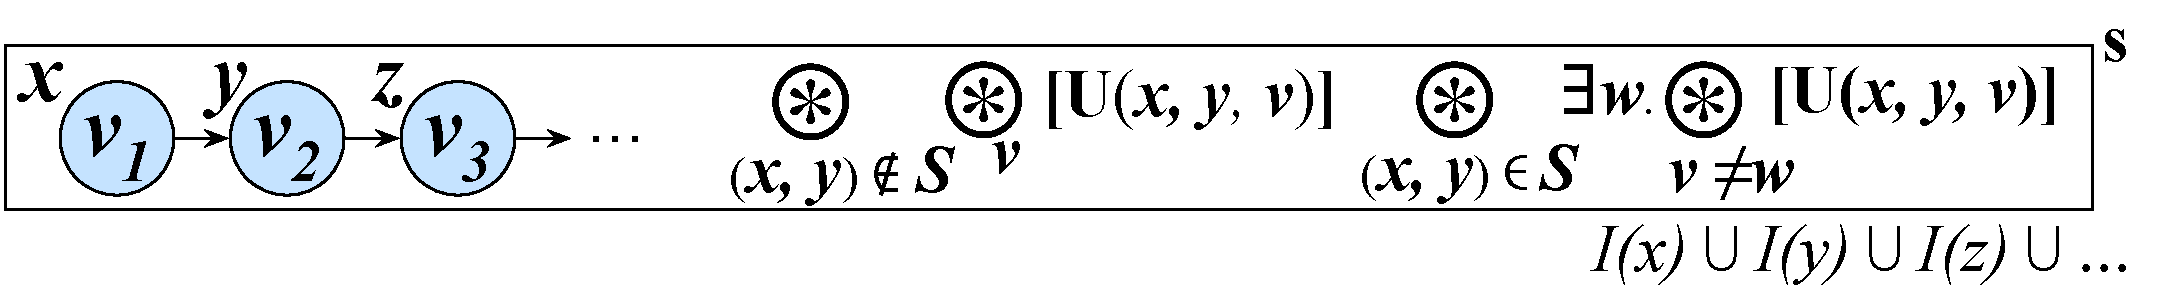
\includegraphics[scale=0.232]{Sections/Examples/Images/capSet.pdf}\\}
%
%
The elements of the list are represented as a singly-linked list with no duplicate elements; the list starts at address $x$ with value $v_1$ and points to the next element at address $y$ with value $v_2$ and so forth. In the remainder of this section, we write $\node{x}{v}{y}$ to denote a node at address $x$, with value $v$ and successor $y$. 

All nodes of the list reside in a single shared region labelled $s$ and the interference on the list is the combined interference associated with each constituent node. 
Each node at a given address $x$ is associated with a set of update capabilities of the form $[\text{U}(x, y, v)]$ for \emph{all} possible addresses $y$ and \emph{all} possible values $v$. This is to capture all potential successor addresses $y$ and all potential values $v$ that may be stored at address $x$. 
%For instance, since the value $v_{1}$ may be contained in the list at address $x$ before address $y$, there must exist an update capability $[\text{U}(x, y, v_1)]$ to accommodate possible modifications of value $v_{1}$ with respect to $x$ and $y$. 
In order to modify a node, a thread can acquire the lock associated with the node and subsequently claim the relevant update capability.
% 

Since in CAP the capabilities associated with a region can only be generated upon region creation, the shared region is required to keep track of all possible update capabilities $[\text{U}(x, y, v)]$ associated with all addresses $x$ (including those not currently in the domain of the list), all addresses $y$ and all values $v$. At any one point, given $\node{x}{v}{y}$, the only update capability that can be claimed by a thread (through locking) is the one that reflects its current status, namely $[\text{U}(x, y, v)]$. As a result, an auxiliary mathematical set $S$ is used to track those nodes of the list that are currently locked and thus infer which $[\text{U}]$ capabilities have been claimed. The distribution of update capabilities is captured by the two assertions written as the \emph{infinite multiplicative star operator} $\iterStar$. The first part of the assertion states that given any node at address $x$ with successor $y$, if it is not locked, i.e.\ $(x, y) \not\in S$, then \emph{all} of its update capabilities of the form $[\text{U}(x, y, v)]$ lie in the shared region for \emph{all} values $v$. Dually, if it is locked, i.e.\ $(x, y) \in S$, then the update capabilities for \emph{all} values $v$ \emph{but one} ($w \not= v$) are in the shared region.

This specification is unnecessarily complicated. It is rather counter-intuitive to account for the capabilities pertaining to addresses not in the domain of the list. Moreover, it is overly verbose to consider all combinations of values and successor addresses. Lastly, each thread is required to ``know'' of the resources associated with all nodes in the list and account for their associated interference. 

%
We proceed with the \colosl\ specification of the set module. Recall from \S\ref{sec:colosl} that \colosl\ is parametric in the separation algebra of capabilities. We thus instantiate it with a heap-like capability separation algebra that is \emph{stateful} and demonstrate that this allows for a more concise specification.  

We specify the set predicate as the $*$-composition of the subjective views pertaining to each node in the singly-linked list as illustrated below. The interference on each subjective view is limited to the node in question. Associated with each node at address $x$ is a ``next'' capability $\nextC{x}{y}$ that tracks its successor $y$. This is analogous to the $[\text{U}(x, y, v)]$ capability of CAP and we shortly demonstrate how it is utilised in our reasoning. Since \colosl\ allows for \emph{dynamic} extension of the shared state, we do not need to account for capabilities associated with \emph{all} possible addresses. Instead, fresh capabilities are generated dynamically as needed. We demonstrate this by giving a reasoning outline of the \li{add(}$v'$\li{)} method. 

%
{\centering 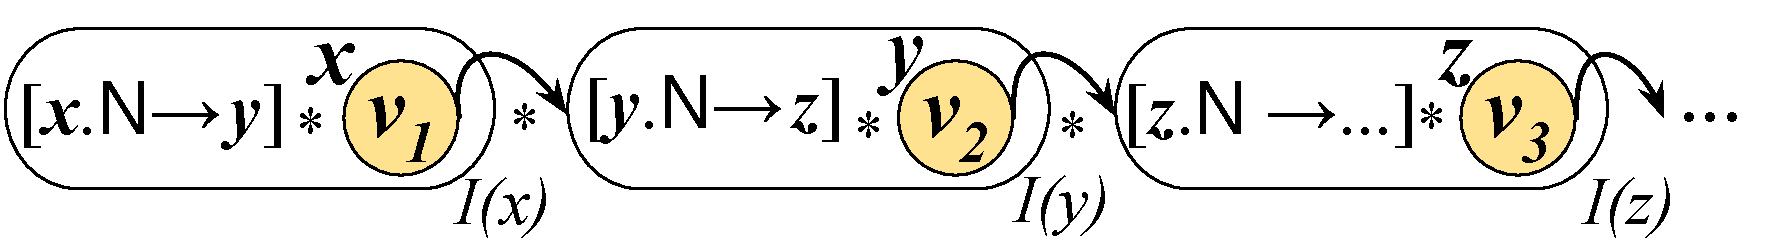
\includegraphics[scale=0.25]{Sections/Examples/Images/coloslSet.pdf}\\}
%
\noindent Suppose $v_2 < v' < v_3$, and thus a new node $w$ with value $v'$ is to be inserted after node $y$.  The operating thread proceeds by traversing the list by hand-over-hand locking until it reaches node $y$. It then locks $y$ and claims its next pointer and moves it to its local state, as allowed by $I(y)$. Subsequently, the shared state is \emph{extended} by the resources associated with the new node ($\cell{w}{v', z}$) and its associated capabilities ($\nextC{w}{z}$) are generated on the fly as depicted below.

%
{\centering 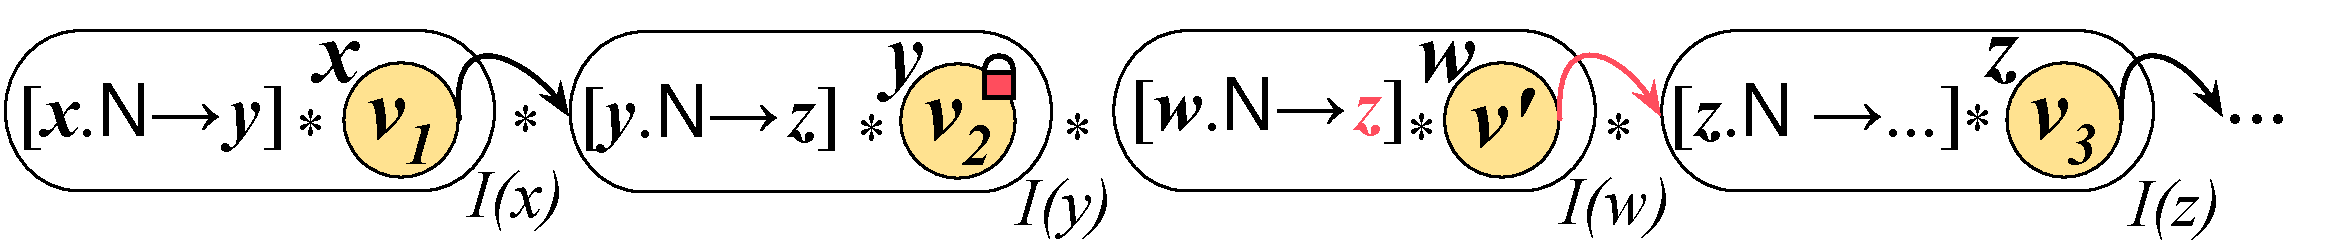
\includegraphics[scale=0.25]{Sections/Examples/Images/add1.pdf}\\}
%
%At this point, since the locking thread holds the next pointer of $y$ in its local state, it modifies it to point to the new node $w$. It then unlocks $y$ and returns its next pointer to the shared state. However, the interference assertion associated with node $y$ ($I(y)$) allows the node to be unlocked in three possible ways. Either its successor has not changed from its old value $z$ (tracked by $\nextC{y}{z}$); \emph{or} it has been redirected to $z$'s successor (when $z$ is being deleted); \emph{or} it has been directed to a new node whose successor is $z$ (a new node is inserted between $y$ and $z$). When adding a new node after $y$, the latter of the possibilities is applicable and thus the unlocking thread must demonstrate that the new node ($w$) does indeed point to $z$. In order to establish this condition, we use the (\mergeRule) principle in our reasoning to combine the subjective views of $y$ and $w$ as follows.
\noindent Since the locking thread holds the next pointer of $y$ in its local state, it modifies it to point to the new node $w$. It then unlocks $y$ and returns its next pointer to the shared state. When inserting a new node between $y$ and $z$, the associated interference assertion ($I(y)$) allows $y$ to be unlocked only if it has been directed to a new node whose successor is $z$. As such, the unlocking thread must demonstrate that the new node ($w$) does indeed point to $z$. In order to establish this, we use the \mergeRule principle to combine the subjective views of $y$ and $w$ as follows.

%
{\centering 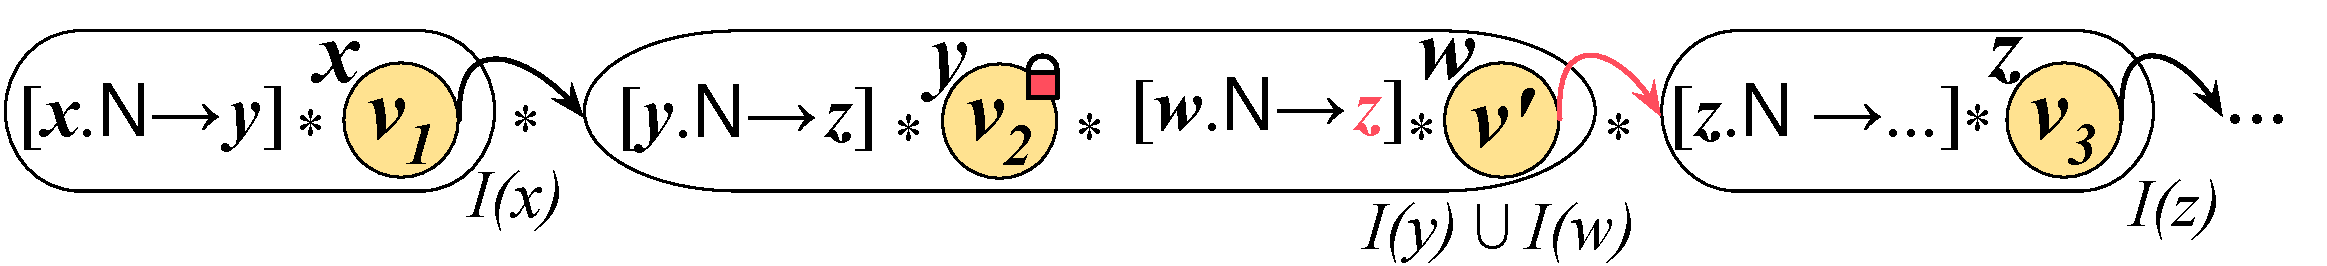
\includegraphics[scale=0.25]{Sections/Examples/Images/add2.pdf}\\}
%
%Finally, node $y$ is unlocked; its updated next pointer is returned to the shared state and its next capability is modified accordingly to reflect its new successor. Using the (\copyRule), (\forgetRule) and (\shiftRule) principles \textit{ad seriatim}, we can once again obtain the set predicate with the new node $w$ inserted. 
\noindent Finally, $y$ is unlocked; its next pointer is returned to the shared state and its next capability is modified to reflect its new successor. Using the \copyRule, \forgetRule and \shiftRule principles \textit{ad seriatim}, we obtain the set predicate with $w$ inserted. 

%
{\centering 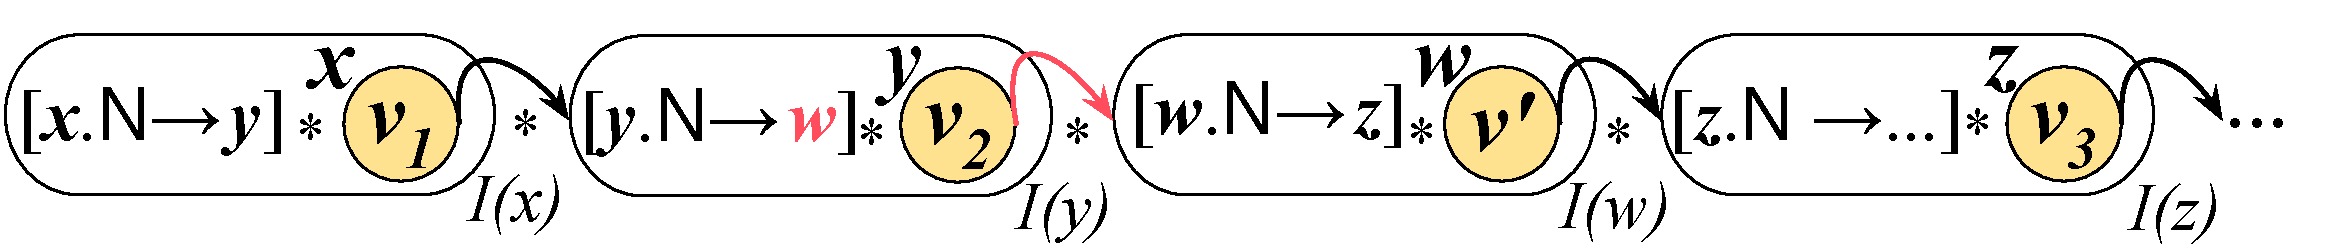
\includegraphics[scale=0.25]{Sections/Examples/Images/add3.pdf}\\}
%
We can reason about the \li{remove} operation in a similar fashion. The dynamic extension afforded by the \extendRule\ principle allows us to generate new capabilities only when needed and thus gives way to a conciser specification. 
%
Moreover, rather than having a distinct capability to modify the element at address $x$, before address $y$, for each possible successor address $y$ (as with $[\text{U}(x, y, v)]$ in CAP), we appeal to a single capability of the form $\nextC{x}{y}$ whereby the capability is modified accordingly to record the changes to the successor address. 
%
Lastly, using the reasoning principles of \mergeRule, \forgetRule, \shiftRule\ and \copyRule, we can grow and shrink our subjective views as needed and consequently at any one point we only view the relevant parts of the shared state. 
%
The full \colosl\ specification of the set module as well as the specification proofs are provided in Appendix~\ref{sec:set-example}.

